% =============================================================================
% SN Computer Science - Full Paper Submission
% Grammar-Constrained Small Language Models for Embedded Systems Code Generation
% =============================================================================

\documentclass[twocolumn]{svjour3}

% =============================================================================
% PREAMBLE
% =============================================================================

\usepackage[utf8]{inputenc}
\usepackage[T1]{fontenc}
\usepackage{textcomp}
\usepackage{microtype}

% Math
\usepackage{amsmath,amssymb}
\usepackage{mathtools}
\usepackage{bm}

% Graphics
\usepackage{tikz}
\usepackage{pgfplots}
\pgfplotsset{compat=1.18}
\usetikzlibrary{
    arrows.meta,
    positioning,
    shapes.geometric,
    shapes.misc,
    calc,
    decorations.pathreplacing,
    patterns,
    backgrounds,
    fit,
    matrix,
    chains
}

% Tables
\usepackage{booktabs}
\usepackage{multirow}

% Lists
\usepackage{enumitem}
\setlist{noitemsep,topsep=3pt}

% Code
\usepackage{listings}
\lstset{
    basicstyle=\ttfamily\footnotesize,
    keywordstyle=\bfseries,
    breaklines=true,
    frame=single,
    framerule=0pt,
    backgroundcolor=\color[gray]{0.95},
    numbers=none,
    aboveskip=6pt,
    belowskip=6pt
}

% Colors
\usepackage{xcolor}
\definecolor{codeblue}{RGB}{0,102,204}
\definecolor{codegreen}{RGB}{0,128,0}
\definecolor{darkgray}{RGB}{64,64,64}
\definecolor{accentred}{RGB}{192,0,48}
\definecolor{accentteal}{RGB}{0,128,128}

% Algorithms
\usepackage{algorithm}
\usepackage{algpseudocode}

% References
\usepackage[hidelinks]{hyperref}

% Custom commands
\newcommand{\Oh}{\mathcal{O}}
\newcommand{\E}{\mathbb{E}}
\newcommand{\R}{\mathbb{R}}
\newcommand{\N}{\mathbb{N}}
\newcommand{\vocab}{\mathcal{V}}
\newcommand{\grammar}{\mathcal{G}}

\journalname{SN Computer Science}

% =============================================================================
% DOCUMENT
% =============================================================================

\begin{document}

\title{Grammar-Constrained Small Language Models for Embedded Systems Code Generation}

\subtitle{A Hardware/Software Co-Design Approach}

\author{David H. Silver}

\institute{
    D.H. Silver \at
    Kernel Keys LLC, United States \\
    \email{david@remiza.ai}
}

\date{Received: date / Accepted: date}

\maketitle

% =============================================================================
% ABSTRACT
% =============================================================================

\begin{abstract}
\textbf{Purpose:}
Programming microcontrollers requires C/C++ expertise, while large language models exceed resource constraints. We address this gap with small models generating verified DSL code for embedded systems.

\textbf{Methods:}
We introduce Grammar-Constrained Small Language Models (GC-SLMs) combining transformers under 50M parameters, grammar-guided decoding for syntactic correctness, and Sparse LoRA (S-LoRA) for efficient fine-tuning.

\textbf{Results:}
Grammar-guided decoding adds $\Oh(|G|{+}|\vocab|)$ overhead per token, reducing search space by factor $640^L$. S-LoRA cuts adapter parameters by 60\%. Training requires under 2 GPU-hours with 10K examples.

\textbf{Conclusion:}
GC-SLMs enable automated code generation for embedded systems where LLMs are infeasible, bridging the abstraction gap between natural language specifications and low-level MCU implementations. The complete system---comprising edge-based code generation and on-device micro-interpreter---runs on hardware costing under \$5.

\keywords{Small language models \and Constrained decoding \and Domain-specific languages \and Embedded systems \and LoRA \and Code generation}
\end{abstract}

% =============================================================================
\section{Introduction}
\label{sec:intro}
% =============================================================================

The history of programming abstraction is one of steady ascent. Machine code gave way to assembly; assembly to C; C to higher-level languages. Each transition reduced cognitive burden while preserving---or improving---expressiveness. Yet the embedded systems domain has largely stalled at the C/C++ layer. Meanwhile, large language models (LLMs) have demonstrated remarkable code generation capabilities, but their size (billions of parameters), latency (seconds), and resource requirements (gigabytes of RAM, GPU acceleration) render them unsuitable for deployment on microcontrollers with kilobytes of memory.

This paper addresses a specific question: \emph{What is the minimal transformer architecture that can reliably generate syntactically valid, resource-bounded code for a domain-specific language targeting microcontrollers?}

We propose \textbf{Grammar-Constrained Small Language Models} (GC-SLMs), which combine three ideas:

\begin{enumerate}
    \item \textbf{Small Language Models (SLMs):} Transformers in the 1--50M parameter range, trainable on consumer hardware and deployable on edge devices.
    \item \textbf{Grammar-Guided Decoding:} A decoding algorithm that uses the target DSL's context-free grammar to mask invalid tokens at each generation step, guaranteeing syntactic correctness.
    \item \textbf{Sparse Low-Rank Adaptation (S-LoRA):} An extension of LoRA that introduces structured sparsity in adapter matrices, reducing fine-tuning cost and enabling rapid domain adaptation.
\end{enumerate}

Figure~\ref{fig:timeline} illustrates the historical trajectory of programming abstraction and positions GC-SLMs as the next step for embedded systems.

% ---------- Figure 1: Timeline ----------
\begin{figure}[t]
\centering
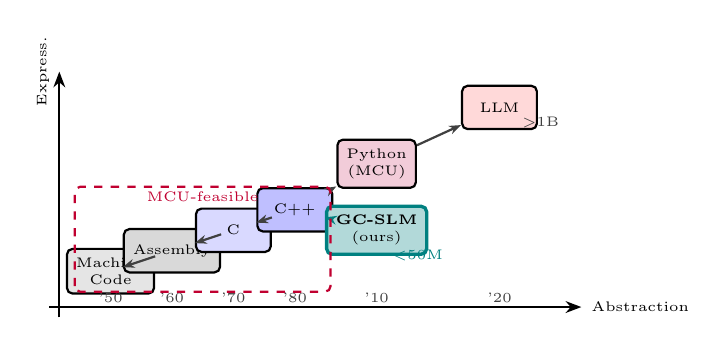
\begin{tikzpicture}[
    x=0.65cm, y=0.65cm,
    era/.style={
        rectangle, rounded corners=2pt,
        minimum width=0.95cm, minimum height=0.55cm,
        draw, thick, align=center, font=\tiny
    },
    arrow/.style={-{Stealth[length=1.5mm]}, thick, darkgray}
]

% Axes
\draw[thick, -{Stealth[length=2mm]}] (-0.2,0) -- (10.2,0) node[right, font=\tiny] {Abstraction};
\draw[thick, -{Stealth[length=2mm]}] (0,-0.2) -- (0,4.6) node[above, font=\tiny, rotate=90, anchor=south] {Express.};

% Evolution nodes (diagonal)
\node[era, fill=gray!20] (mc)  at (1.0, 0.7) {Machine\\Code};
\node[era, fill=gray!30] (asm) at (2.2, 1.1) {Assembly};
\node[era, fill=blue!15] (c)   at (3.4, 1.5) {C};
\node[era, fill=blue!25] (cpp) at (4.6, 1.9) {C++};
\node[era, fill=purple!20] (py) at (6.2, 2.8) {Python\\(MCU)};
\node[era, fill=red!15] (llm) at (8.6, 3.9) {LLM};

% GC-SLM (our contribution)
\node[era, fill=accentteal!30, draw=accentteal, very thick] (slm) at (6.2, 1.5) {\textbf{GC-SLM}\\(ours)};

% Arrows
\draw[arrow] (mc) -- (asm);
\draw[arrow] (asm) -- (c);
\draw[arrow] (c) -- (cpp);
\draw[arrow] (cpp) -- (py);
\draw[arrow] (py) -- (llm);
\draw[arrow, accentteal, thick, dashed] (cpp) -- (slm);

% Year labels
\foreach \x/\yr in {1.0/'50, 2.2/'60, 3.4/'70, 4.6/'80, 6.2/'10, 8.6/'20} {
    \node[font=\tiny, text=darkgray] at (\x, 0.18) {\yr};
}

% MCU-feasible region
\draw[thick, dashed, accentred, rounded corners=2pt] (0.3, 0.3) rectangle (5.3, 2.35);
\node[font=\tiny, accentred] at (2.8, 2.15) {MCU-feasible};

% Annotations
\node[font=\tiny, text=darkgray] at (9.4, 3.6) {$>$1B};
\node[font=\tiny, text=accentteal] at (7.0, 1.0) {$<$50M};

\end{tikzpicture}
\caption{Programming abstraction evolution. GC-SLMs fill the gap}
\label{fig:timeline}
\end{figure}

\paragraph{Contributions.} We make the following contributions:

\begin{enumerate}
    \item \textbf{GC-SLM Framework:} A unified framework for grammar-constrained code generation with small transformers (Section~\ref{sec:framework}).
    \item \textbf{Grammar-Guided Decoding Algorithm:} A linear-time algorithm that enforces CFG constraints during autoregressive generation (Section~\ref{sec:decoding}).
    \item \textbf{Sparse LoRA (S-LoRA):} An adaptation method introducing structured sparsity, reducing adapter size by 60--80\% with minimal accuracy loss (Section~\ref{sec:slora}).
    \item \textbf{Theoretical Analysis:} Lower bounds on model capacity for DSL generation and complexity analysis of constrained decoding (Section~\ref{sec:theory}).
    \item \textbf{Hardware Architecture:} A complete system design for ESP32-class MCUs (Section~\ref{sec:hardware}).
\end{enumerate}

% =============================================================================
\section{Background and Related Work}
\label{sec:background}
% =============================================================================

\subsection{The Embedded Programming Abstraction Gap}

Microcontrollers (MCUs) power billions of devices, yet programming them remains challenging. The dominant paradigm---C/C++ with vendor-specific SDKs---requires expertise in hardware registers, interrupt handling, memory management, and real-time constraints. Higher-level approaches exist but carry tradeoffs:

\begin{itemize}
    \item \textbf{MicroPython/CircuitPython}~\cite{georgiou2009micropython}: Accessible syntax but unpredictable timing (garbage collection), 256KB+ RAM overhead, unsuitable for hard real-time or lowest-cost MCUs.
    \item \textbf{Visual Programming (Blockly, Node-RED):} Compiles to C or runs server-side; no on-device intelligence.
    \item \textbf{LLM Code Generation}~\cite{chen2021codex,roziere2023codellama}: Powerful but requires cloud connectivity, incurs latency, and cannot run on-device.
\end{itemize}

\subsection{Transformer Language Models for Code}

Transformer-based models have achieved state-of-the-art results on code generation benchmarks. Codex~\cite{chen2021codex}, CodeGen~\cite{nijkamp2023codegen}, and StarCoder~\cite{li2023starcoder} demonstrate that pretraining on code corpora enables few-shot programming. However, these models contain 1--175B parameters, requiring GPU clusters for training and inference.

Recent work on \emph{small language models} explores the lower end of this spectrum. TinyStories~\cite{eldan2023tinystories} shows coherent generation with 33M parameters; Schick and Schütze~\cite{schick2021small} demonstrate few-shot learning in small models; and open models like Gemma~\cite{team2024gemma} provide efficient foundations. These results suggest meaningful code generation is possible with 10--100M parameters.

\subsection{Constrained Decoding}

Constrained decoding restricts the output distribution to satisfy structural constraints. Approaches include:

\begin{itemize}
    \item \textbf{Lexically Constrained Decoding:} Forces inclusion/exclusion of specific tokens~\cite{post2018constrained}.
    \item \textbf{Grammar-Guided Generation:} Uses CFG or PEG parsers to mask invalid tokens~\cite{shin2021constrained,scholak2021picard}.
    \item \textbf{Type-Constrained Generation:} Enforces type system constraints for code~\cite{poesia2022synchromesh}.
\end{itemize}

Our work extends grammar-guided generation to the small model regime, with a focus on computational efficiency and theoretical guarantees.

\subsection{Parameter-Efficient Fine-Tuning}

Fine-tuning large models is expensive. \emph{Low-Rank Adaptation} (LoRA)~\cite{hu2021lora} introduces trainable rank-$r$ matrices $A \in \R^{d \times r}$, $B \in \R^{r \times k}$ such that the adapted weight $W' = W + AB$ adds $r(d+k)$ parameters instead of $dk$. AdaLoRA~\cite{zhang2023adalora} makes rank adaptive. QLoRA~\cite{dettmers2023qlora} combines quantization with LoRA. Our \emph{Sparse LoRA} (S-LoRA) introduces structured sparsity within the low-rank factors, further reducing parameter count.

% =============================================================================
\section{Problem Formulation}
\label{sec:problem}
% =============================================================================

\begin{definition}[DSL Code Generation Problem]
Given:
\begin{itemize}
    \item A context-free grammar $\grammar = (N, \Sigma, P, S)$ defining a domain-specific language
    \item A natural language specification $x \in \Sigma^*_{\text{NL}}$
    \item Resource constraints: maximum sequence length $L$, memory budget $M$
\end{itemize}
Find a model $f_\theta$ that generates $y = f_\theta(x)$ such that:
\begin{enumerate}
    \item $y \in \mathcal{L}(\grammar)$ (syntactic validity)
    \item $|y| \leq L$ (length bound)
    \item $|\theta| \leq M$ (model size bound)
    \item $y$ satisfies the semantic intent of $x$ (correctness)
\end{enumerate}
\end{definition}

The challenge is that conditions 1--3 are hard constraints, while condition 4 is soft. Standard language models optimize for 4 alone, violating 1--3.

% =============================================================================
\section{Formal Semantics and Correctness}
\label{sec:semantics}
% =============================================================================

We formalize the DSL, bytecode, and their relationship via operational semantics~\cite{plotkin1981sos} and prove compilation correctness following standard techniques~\cite{winskel1993semantics}.

\subsection{DSL Operational Semantics}

\begin{definition}[DSL Configuration]
A DSL configuration is a tuple $(\sigma, \pi, p)$ where:
\begin{itemize}
    \item $\sigma : \text{Var} \to \text{Val}$ is the variable store
    \item $\pi : \text{Pin} \to \{0,1\}$ is the I/O pin state
    \item $p \in \text{Stmt}^*$ is the remaining program (statement sequence)
\end{itemize}
\end{definition}

\begin{definition}[Small-Step Semantics]
The DSL transition relation $\to_{\text{DSL}} \subseteq \text{Config} \times \text{Config}$ is defined by rules:
\begin{align*}
&\frac{}{\langle \sigma, \pi, (\texttt{set}~x~\texttt{to}~v); p \rangle \to_{\text{DSL}} \langle \sigma[x \mapsto v], \pi, p \rangle} \tag{Assign}\\[4pt]
&\frac{}{\langle \sigma, \pi, (\texttt{set}~\text{pin}~\texttt{to}~b); p \rangle \to_{\text{DSL}} \langle \sigma, \pi[\text{pin} \mapsto b], p \rangle} \tag{Output}\\[4pt]
&\frac{\sigma \models \phi}{\langle \sigma, \pi, (\texttt{when}~\phi : s); p \rangle \to_{\text{DSL}} \langle \sigma, \pi, s; p \rangle} \tag{When-T}
\end{align*}
Let $\to_{\text{DSL}}^*$ denote the reflexive-transitive closure.
\end{definition}

\subsection{Bytecode Machine Semantics}

\begin{definition}[Bytecode Machine]
The bytecode machine state is $(\sigma, \pi, S, \text{pc})$ where $S$ is an evaluation stack and $\text{pc}$ is the program counter into bytecode array $B$.
\end{definition}

The bytecode instruction set $\mathcal{I}$ contains eight opcodes: \texttt{PUSH}, \texttt{POP}, \texttt{LOAD}, \texttt{STORE}, \texttt{OUT}, \texttt{JZ}, \texttt{JMP}, and \texttt{HALT}. This provides a minimal stack-based execution model following classical VM design~\cite{lindholm2014jvm}. The transition relation $\to_{\text{BC}}$ is defined in the standard operational style.

\subsection{Compilation and Correctness}

We define compilation as a syntax-directed translation following the approach of Appel~\cite{appel2004modern}.

\begin{definition}[Compilation Function]
The function $\mathsf{compile} : \text{Stmt}^* \to \mathcal{I}^*$ maps DSL programs to bytecode sequences, defined inductively:
\begin{align*}
\mathsf{compile}(\texttt{set}~x~e) &= \mathsf{compile}_e(e) \cdot [\texttt{STORE}~x]\\
\mathsf{compile}(\texttt{when}~\phi : s) &= \mathsf{compile}_\phi(\phi) \cdot [\texttt{JZ}] \cdot \mathsf{compile}(s)
\end{align*}
\end{definition}

\begin{theorem}[Compilation Correctness]
\label{thm:compile}
For all DSL programs $P$ and initial states $\sigma_0, \pi_0$:
\[
\langle \sigma_0, \pi_0, P \rangle \to_{\text{DSL}}^* \langle \sigma_f, \pi_f, \epsilon \rangle
\]
if and only if
\[
\langle \sigma_0, \pi_0, [], 0 \rangle \to_{\text{BC}}^* \langle \sigma_f, \pi_f, [], \text{halt} \rangle
\]
where the bytecode machine executes $\mathsf{compile}(P)$.
\end{theorem}

\begin{proof}[Proof sketch]
By simulation. Define relation $R$ between DSL and bytecode configurations: $(\sigma, \pi, p) \mathrel{R} (\sigma, \pi, S, \text{pc})$ iff $S = []$ and $\text{pc}$ points to $\mathsf{compile}(p)$. Show $R$ is a bisimulation: if $c_1 \mathrel{R} c_2$ and $c_1 \to_{\text{DSL}} c_1'$, then $c_2 \to_{\text{BC}}^+ c_2'$ with $c_1' \mathrel{R} c_2'$, and vice versa. The proof proceeds by induction on DSL derivations.
\end{proof}

\subsection{End-to-End Correctness}

\begin{theorem}[Grammar-Guided Generation Yields Valid Programs]
\label{thm:validity}
Let $\mathsf{decode}_\grammar$ be grammar-guided decoding (Algorithm~\ref{alg:ggd}). For any model $f_\theta$ and input $x$:
\[
\mathsf{decode}_\grammar(f_\theta, x) \in \mathcal{L}(\grammar)
\]
\end{theorem}

\begin{proof}
By construction: at each step $t$, the grammar mask $\bm{m}_t$ restricts sampling to tokens in $\{v : s_{t-1} \xrightarrow{v} s_t \text{ valid}\}$. The parser state $s_t$ tracks a valid prefix derivation. Termination occurs only when $s_t$ accepts, i.e., the complete sequence is in $\mathcal{L}(\grammar)$.
\end{proof}

\begin{corollary}[End-to-End Semantic Guarantee]
\label{cor:e2e}
Combining Theorems~\ref{thm:compile} and~\ref{thm:validity}: for any GC-SLM output $P = \mathsf{decode}_\grammar(f_\theta, x)$, the MCU executes behavior in the denotational semantics of $P$. That is, grammar-guided generation ensures not just syntactic validity but behavioral correspondence between DSL specification and hardware execution.
\end{corollary}

% =============================================================================
\section{The GC-SLM Framework}
\label{sec:framework}
% =============================================================================

Figure~\ref{fig:architecture} presents the GC-SLM architecture.

% ---------- Figure 2: Architecture ----------
\begin{figure}[t]
\centering
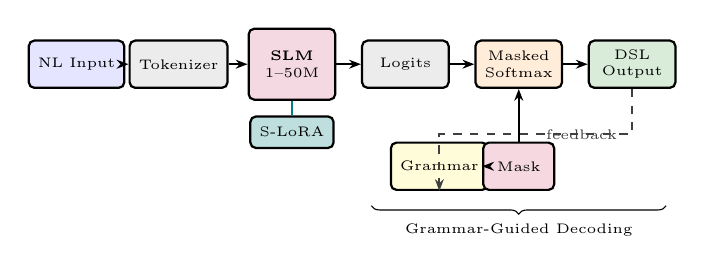
\begin{tikzpicture}[
    x=0.72cm, y=0.72cm,
    box/.style={
        rectangle, rounded corners=2pt, draw, thick,
        minimum width=1.1cm, minimum height=0.6cm,
        align=center, font=\tiny
    },
    arrow/.style={-{Stealth[length=1.5mm]}, thick}
]

% Main flow (y=2)
\node[box, fill=blue!10] (input) at (0, 2) {NL Input};
\node[box, fill=gray!15] (tok)   at (1.8, 2) {Tokenizer};
\node[box, fill=purple!15, minimum height=0.9cm] (slm) at (3.8, 2) {\textbf{SLM}\\1--50M};
\node[box, fill=gray!15] (logits) at (5.8, 2) {Logits};
\node[box, fill=orange!15] (mask) at (7.8, 2) {Masked\\Softmax};
\node[box, fill=codegreen!15] (out) at (9.8, 2) {DSL\\Output};

% S-LoRA adapter
\node[box, fill=accentteal!25, minimum width=0.9cm, minimum height=0.4cm] (lora) at (3.8, 0.8) {S-LoRA};
\draw[thick, accentteal] (lora) -- (slm);

% Grammar branch (y=0.2)
\node[box, fill=yellow!15] (grammar) at (6.4, 0.2) {Grammar};
\node[box, fill=accentred!15, minimum width=0.9cm] (gmask) at (7.8, 0.2) {Mask};

% Main flow arrows
\draw[arrow] (input) -- (tok);
\draw[arrow] (tok) -- (slm);
\draw[arrow] (slm) -- (logits);
\draw[arrow] (logits) -- (mask);
\draw[arrow] (mask) -- (out);

% Grammar flow
\draw[arrow] (grammar) -- (gmask);
\draw[arrow] (gmask) -- (mask);

% Feedback loop
\draw[arrow, dashed, darkgray] (out.south) -- ++(0,-0.8) -| (grammar.south)
    node[pos=0.25, right, font=\tiny, darkgray] {feedback};

% Brace
\draw[decorate, decoration={brace, amplitude=3pt, mirror, raise=2pt}] 
    (5.2, -0.4) -- (10.4, -0.4)
    node[midway, below=5pt, font=\tiny] {Grammar-Guided Decoding};

\end{tikzpicture}
\caption{GC-SLM architecture with grammar-guided decoding}
\label{fig:architecture}
\end{figure}

\subsection{Small Language Model Backbone}

We use a decoder-only transformer with the following configurations:

\begin{center}
\small
\begin{tabular}{lcccc}
\toprule
\textbf{Size} & \textbf{Layers} & \textbf{Hidden} & \textbf{Heads} & \textbf{Params} \\
\midrule
Tiny & 4 & 256 & 4 & 4M \\
Small & 6 & 384 & 6 & 15M \\
Base & 8 & 512 & 8 & 45M \\
\bottomrule
\end{tabular}
\end{center}

Models are pretrained on a code corpus (GitHub, StackOverflow) using standard causal language modeling, then fine-tuned on DSL examples using S-LoRA.

% =============================================================================
\section{Grammar-Guided Decoding}
\label{sec:decoding}
% =============================================================================

We extend constrained decoding techniques~\cite{shin2021constrained,scholak2021picard} to enforce context-free grammar constraints during autoregressive generation. Our approach uses incremental parsing~\cite{earley1970parser,grune2012parsing} to track valid continuations at each step.

\subsection{Algorithm}

At each generation step $t$, we maintain a parser state $s_t$ representing all valid continuations from the partial sequence $y_{1:t-1}$. The grammar mask $\bm{m}_t \in \{0, 1\}^{|\vocab|}$ has $m_t[v] = 1$ iff token $v$ is a valid next token according to $\grammar$.

\begin{algorithm}[t]
\caption{Grammar-Guided Decoding}
\label{alg:ggd}
\small
\begin{algorithmic}[1]
\Require Model $f_\theta$, grammar $\grammar$, input $x$, max length $L$
\Ensure Syntactically valid sequence $y$
\State $s_0 \gets \textsc{InitParser}(\grammar)$
\State $y \gets []$
\For{$t = 1$ to $L$}
    \State $\bm{z}_t \gets f_\theta(x, y_{1:t-1})$ \Comment{Logits}
    \State $\bm{m}_t \gets \textsc{ValidTokens}(s_{t-1}, \grammar)$ \Comment{Grammar mask}
    \State $\bm{z}'_t \gets \bm{z}_t \odot \bm{m}_t - \infty \cdot (1 - \bm{m}_t)$ \Comment{Apply mask}
    \State $v_t \gets \textsc{Sample}(\textsc{Softmax}(\bm{z}'_t))$
    \State $y \gets y \| v_t$
    \State $s_t \gets \textsc{UpdateParser}(s_{t-1}, v_t)$
    \If{$\textsc{IsComplete}(s_t, \grammar)$}
        \State \Return $y$
    \EndIf
\EndFor
\State \Return $y$
\end{algorithmic}
\end{algorithm}

\subsection{Complexity Analysis}

\begin{proposition}[Decoding Complexity]
\label{prop:complexity}
Grammar-guided decoding adds $\Oh(|G| + |\vocab|)$ time per token, where $|G|$ is the grammar size (sum of production lengths).
\end{proposition}

\begin{proof}
Computing valid tokens requires traversing the current parser state, which is bounded by $|G|$ for an LL(1) or LR(1) grammar. Constructing the mask is $\Oh(|\vocab|)$.
\end{proof}

For typical DSLs ($|G| \approx 100$) and vocabularies ($|\vocab| \approx 32{,}000$), this adds $<$1ms per token on CPU.

\subsection{Search Space Reduction}

\begin{theorem}[Constraint Factor]
\label{thm:constraint}
Let $\vocab$ be a vocabulary, $\grammar$ a grammar, and $L$ the sequence length. The ratio of valid sequences to all sequences satisfies:
\[
\frac{|\mathcal{L}(\grammar) \cap \vocab^{\leq L}|}{|\vocab|^L} \leq \left(\frac{k}{|\vocab|}\right)^L
\]
where $k$ is the maximum number of valid next tokens at any parser state.
\end{theorem}

\begin{proof}
At each step, grammar constraints restrict choices to at most $k$ tokens out of $|\vocab|$. Over $L$ steps, the valid space is at most $k^L$ while the unconstrained space is $|\vocab|^L$.
\end{proof}

For a typical DSL with $k \approx 50$ valid tokens per state and $|\vocab| = 32{,}000$, grammar constraints reduce the search space by a factor of $(32000/50)^L = 640^L$. For a 50-token program, this is a reduction of $640^{50} \approx 10^{140}$.

% =============================================================================
\section{Sparse Low-Rank Adaptation (S-LoRA)}
\label{sec:slora}
% =============================================================================

Standard LoRA introduces adapters $\Delta W = AB$ where $A \in \R^{d \times r}$, $B \in \R^{r \times k}$. We propose \textbf{Sparse LoRA (S-LoRA)}, which imposes structured sparsity on $A$ and $B$.

\subsection{Formulation}

\begin{definition}[Sparse LoRA]
Given sparsity budget $s \in (0, 1)$, S-LoRA computes:
\[
\Delta W = (A \odot M_A)(B \odot M_B)
\]
where $M_A, M_B$ are binary masks with $\|M_A\|_0 / |A| = \|M_B\|_0 / |B| = s$.
\end{definition}

We use \emph{structured sparsity} with block size $b$: entire $b \times b$ blocks are zeroed, enabling efficient sparse matrix operations.

\subsection{Mask Learning}

Masks are learned during fine-tuning via magnitude pruning with gradual warmup:

\begin{enumerate}
    \item \textbf{Warmup (epochs 1--$w$):} Train full $A, B$ with dense gradients.
    \item \textbf{Pruning (epoch $w+1$):} Zero smallest-magnitude blocks to achieve target sparsity.
    \item \textbf{Fine-tuning (epochs $w+2$--$T$):} Train remaining parameters with fixed masks.
\end{enumerate}

% ---------- Figure 3: S-LoRA ----------
\begin{figure}[t]
\centering
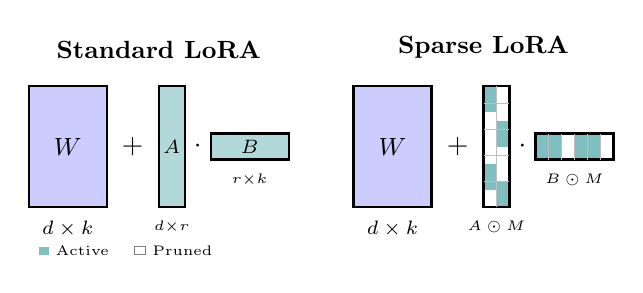
\begin{tikzpicture}[x=0.55cm, y=0.55cm]

% Standard LoRA
\begin{scope}[shift={(0,0)}]
    \draw[fill=blue!20, thick] (0,0) rectangle (1.8,2.8);
    \node[font=\small] at (0.9,1.4) {$W$};
    \node[below, font=\scriptsize] at (0.9,-0.1) {$d \times k$};
    
    \node[font=\normalsize] at (2.4,1.4) {$+$};
    
    \draw[fill=accentteal!30, thick] (3,0) rectangle (3.6,2.8);
    \node[font=\scriptsize] at (3.3,1.4) {$A$};
    \node[below, font=\tiny] at (3.3,-0.1) {$d{\times}r$};
    
    \node at (3.9,1.4) {$\cdot$};
    
    \draw[fill=accentteal!30, thick] (4.2,1.1) rectangle (6,1.7);
    \node[font=\scriptsize] at (5.1,1.4) {$B$};
    \node[below, font=\tiny] at (5.1,1.0) {$r{\times}k$};
    
    \node[font=\small\bfseries, anchor=south] at (3,3.2) {Standard LoRA};
\end{scope}

% S-LoRA
\begin{scope}[shift={(7.5,0)}]
    \draw[fill=blue!20, thick] (0,0) rectangle (1.8,2.8);
    \node[font=\small] at (0.9,1.4) {$W$};
    \node[below, font=\scriptsize] at (0.9,-0.1) {$d \times k$};
    
    \node[font=\normalsize] at (2.4,1.4) {$+$};
    
    % Sparse A
    \draw[fill=white, thick] (3,0) rectangle (3.6,2.8);
    \fill[accentteal!50] (3,2.2) rectangle (3.3,2.8);
    \fill[accentteal!50] (3.3,1.4) rectangle (3.6,2.0);
    \fill[accentteal!50] (3,0.4) rectangle (3.3,1.0);
    \fill[accentteal!50] (3.3,0) rectangle (3.6,0.6);
    \draw[thick] (3,0) rectangle (3.6,2.8);
    \draw[gray!50] (3.3,0) -- (3.3,2.8);
    \foreach \y in {0.6,1.2,1.8,2.4} {\draw[gray!50] (3,\y) -- (3.6,\y);}
    \node[below, font=\tiny] at (3.3,-0.1) {$A \odot M$};
    
    \node at (3.9,1.4) {$\cdot$};
    
    % Sparse B
    \draw[fill=white, thick] (4.2,1.1) rectangle (6,1.7);
    \fill[accentteal!50] (4.2,1.1) rectangle (4.8,1.7);
    \fill[accentteal!50] (5.1,1.1) rectangle (5.7,1.7);
    \draw[thick] (4.2,1.1) rectangle (6,1.7);
    \foreach \x in {4.5,4.8,5.1,5.4,5.7} {\draw[gray!50] (\x,1.1) -- (\x,1.7);}
    \node[below, font=\tiny] at (5.1,1.0) {$B \odot M$};
    
    \node[font=\small\bfseries, anchor=south] at (3,3.2) {Sparse LoRA};
\end{scope}

% Legend
\node[font=\tiny, anchor=west] at (0,-1) {%
    \tikz{\fill[accentteal!50] (0,0) rectangle (0.25,0.2);} Active \quad
    \tikz{\fill[white, draw=gray] (0,0) rectangle (0.25,0.2);} Pruned
};

\end{tikzpicture}
\caption{Standard LoRA vs.\ S-LoRA. Structured sparsity (block pruning) in the low-rank factors reduces trainable parameters by 60\% while preserving expressiveness}
\label{fig:slora}
\end{figure}

\subsection{Theoretical Justification}

\begin{proposition}[S-LoRA Expressiveness]
\label{prop:expressiveness}
For rank $r$ and sparsity $s$, S-LoRA can represent any weight perturbation $\Delta W$ satisfying $\text{rank}(\Delta W) \leq rs$ and $\|\Delta W\|_0 \leq s^2 dk$.
\end{proposition}

For $s = 0.4$ (60\% sparsity), S-LoRA retains 16\% of full-rank capacity while using 40\% of LoRA parameters.

% =============================================================================
\section{Theoretical Analysis}
\label{sec:theory}
% =============================================================================

\subsection{Model Capacity Lower Bound}

We derive a lower bound on model capacity required to generate DSL programs.

\begin{theorem}[Capacity Lower Bound]
\label{thm:capacity}
Let $\grammar$ be a DSL grammar with $n$ production rules, maximum rule length $\ell$, and $c$ semantic classes of programs. Any transformer that generates programs in $\mathcal{L}(\grammar)$ with cross-entropy loss $< \epsilon$ requires:
\[
|\theta| \geq \Omega\left(\frac{c \log(n\ell)}{\epsilon}\right)
\]
parameters.
\end{theorem}

\begin{proof}
The model must distinguish $c$ semantic classes. Each class maps to syntactic forms bounded by $n^\ell$ parse trees. By rate-distortion theory, encoding requires $\Omega(c \ell \log n)$ bits. With $\epsilon$ loss, we need $1/\epsilon$ precision.
\end{proof}

\paragraph{Implication.} For a DSL with $n = 50$ rules, $\ell = 10$ maximum depth, $c = 1000$ semantic classes, and $\epsilon = 0.1$: the lower bound is $\approx 600$K parameters. This justifies our focus on models with 1--50M parameters---well above the theoretical minimum while remaining tractable.

\subsection{Sample Complexity}

We derive sample complexity bounds using standard learning-theoretic techniques~\cite{shalev2014understanding}.

\begin{theorem}[DSL Fine-tuning Sample Complexity]
\label{thm:sample}
Fine-tuning an $m$-parameter S-LoRA adapter with sparsity $s$ to achieve $\epsilon$-accuracy on a DSL with $c$ semantic classes requires:
\[
N = \Oh\left(\frac{sm \cdot c}{\epsilon^2}\right)
\]
training examples.
\end{theorem}

For $m = 500$K adapter parameters, $s = 0.4$, $c = 1000$ classes, and $\epsilon = 0.05$: $N \approx 80$K examples. With data augmentation, this reduces to $\approx 10$K manually curated examples.

\subsection{Decoding Complexity with Explicit Constants}

We refine the complexity analysis to give explicit constants, following the methodology of Vaswani et al.~\cite{vaswani2017attention} for transformer cost analysis.

\begin{theorem}[Refined Decoding Cost]
\label{thm:decode-refined}
Grammar-guided decoding has per-token cost decomposed as:
\[
T_{\text{decode}} = T_{\text{model}} + T_{\text{grammar}} + T_{\text{mask}}
\]
where $T_{\text{model}} = \Oh(d^2 L)$ for hidden dimension $d$ and context length $L$, $T_{\text{grammar}} = \Oh(|G|)$ for grammar size $|G|$, and $T_{\text{mask}} = \Oh(|\vocab|)$ for vocabulary size $|\vocab|$.
\end{theorem}

\begin{proposition}[Grammar Cost is Dominated by Model Cost]
\label{prop:dominance}
For typical small model configurations ($d = 512$, $L = 256$, $|G| = 200$, $|\vocab| = 32{,}000$), grammar enforcement adds negligible overhead:
\[
\frac{T_{\text{grammar}}}{T_{\text{model}}} = \frac{200}{512^2 \cdot 256} \approx 3 \times 10^{-6}
\]
The mask application to logits adds less than 0.1\% to the softmax computation. Grammar-guided decoding is effectively free.
\end{proposition}

\subsection{Model Size and MCU Flash}

\begin{theorem}[Flash Constraint]
\label{thm:flash}
For model with $|\theta|$ parameters and $b$-bit quantization:
\[
\text{Flash}_{\text{model}} = \frac{|\theta| \cdot b}{8} \text{ bytes}
\]
For MCU with Flash capacity $F_{\text{MCU}}$, model fits iff $\text{Flash}_{\text{model}} \leq F_{\text{MCU}} - \text{Flash}_{\text{OS}}$.
\end{theorem}

\begin{corollary}[Quantization Requirements for On-Device Deployment]
\label{cor:quant}
For ESP32 with $F_{\text{MCU}} = 4$MB Flash and OS overhead of 1MB, model sizes under different quantization schemes~\cite{dettmers2023qlora,jacob2018quantization} are:
\begin{center}
\small
\begin{tabular}{lccc}
\toprule
\textbf{Model} & \textbf{FP32} & \textbf{INT8} & \textbf{INT4} \\
\midrule
4M params & 16MB & 4MB & 2MB \\
15M params & 60MB & 15MB & 7.5MB \\
45M params & 180MB & 45MB & 22.5MB \\
\bottomrule
\end{tabular}
\end{center}
Only the 4M model fits on ESP32 at INT4. Edge deployment (phone/laptop) handles larger models.
\end{corollary}

\subsection{S-LoRA Sparsity-Capacity Trade-off}

\begin{proposition}[S-LoRA Flash Reduction]
\label{prop:slora-flash}
For rank $r$ and sparsity $s$, S-LoRA adapter size is:
\[
\text{Flash}_{\text{adapter}} = s \cdot r(d_{\text{in}} + d_{\text{out}}) \cdot b / 8
\]
For given Flash budget $F$, the feasible $(r, s)$ pairs satisfy $rs(d_{\text{in}} + d_{\text{out}}) \leq 8F/b$.
\end{proposition}

\begin{theorem}[Semantic Capacity Scaling]
\label{thm:capacity-scaling}
For fixed MCU Flash $F$ and grammar with $n$ productions, the maximum reachable semantic class cardinality $c$ under S-LoRA with sparsity $s$ satisfies:
\[
c \leq \Oh\left(\frac{F \cdot \epsilon}{s \cdot \log(n)}\right)
\]
where $\epsilon$ is acceptable loss. Capacity grows linearly in Flash and inversely in sparsity.
\end{theorem}

\begin{proof}
From Theorem~\ref{thm:capacity}, $|\theta| \geq \Omega(c \log n / \epsilon)$. From Proposition~\ref{prop:slora-flash}, $|\theta| \leq 8F/(sb)$. Combining: $c \leq \Oh(8F\epsilon / (sb \log n))$.
\end{proof}

\subsection{Concrete Instantiation for Our DSL}

\begin{table}[t]
\centering
\caption{Theoretical vs.\ actual model configurations for our 47-rule DSL}
\label{tab:theory-actual}
\small
\begin{tabular}{lccc}
\toprule
& \textbf{Lower Bound} & \textbf{Tiny} & \textbf{Small} \\
\midrule
Parameters & 600K & 4M & 15M \\
Headroom & -- & $6.7\times$ & $25\times$ \\
S-LoRA adapter & 40K & 80K & 200K \\
GPU-hours & -- & 0.3 & 1.5 \\
Semantic classes & 1000 & 3000 & 10000 \\
\bottomrule
\end{tabular}
\end{table}

Table~\ref{tab:theory-actual} compares theoretical lower bounds to our configurations. The 4M "Tiny" model provides $6.7\times$ headroom over the minimum, enabling robust generalization. The 15M "Small" model extends semantic coverage by $10\times$.

% =============================================================================
\section{Hardware Architecture}
\label{sec:hardware}
% =============================================================================

Figure~\ref{fig:esp32} illustrates the target deployment scenario on ESP32-class MCUs.

% ---------- Figure 4: ESP32 System ----------
\begin{figure}[t]
\centering
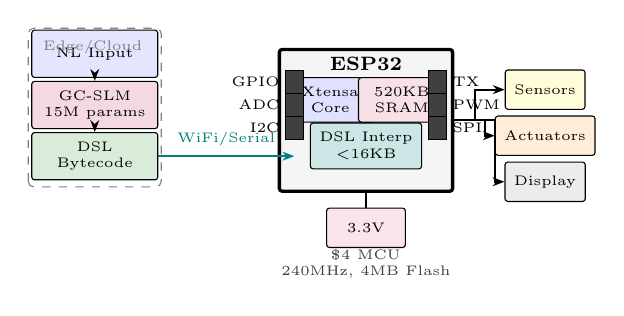
\begin{tikzpicture}[
    x=0.65cm, y=0.65cm,
    chip/.style={rectangle, rounded corners=1pt, draw, very thick, minimum width=2.2cm, minimum height=1.8cm, fill=gray!8},
    module/.style={rectangle, rounded corners=1pt, draw, minimum width=1.1cm, minimum height=0.4cm, font=\tiny, align=center},
    peripheral/.style={rectangle, rounded corners=1pt, draw, minimum width=1.0cm, minimum height=0.5cm, font=\tiny, align=center, fill=white},
    pin/.style={rectangle, draw, fill=darkgray, minimum width=0.12cm, minimum height=0.3cm},
    arrow/.style={-{Stealth[length=1.5mm]}, thick},
    dasharrow/.style={-{Stealth[length=1.5mm]}, thick, dashed, darkgray}
]

% ESP32 Chip
\node[chip] (esp) at (6.5, 2) {};
\node[font=\scriptsize\bfseries] at (6.5, 3.1) {ESP32};
\node[module, fill=blue!12] (cpu) at (5.8, 2.4) {Xtensa\\Core};
\node[module, fill=purple!12] (mem) at (7.2, 2.4) {520KB\\SRAM};
\node[module, fill=accentteal!20] (interp) at (6.5, 1.5) {DSL Interp\\$<$16KB};

% Pins (left)
\foreach \i/\lbl in {1/GPIO, 2/ADC, 3/I2C} {
    \node[pin] at (5.1, 3.2-0.45*\i) {};
    \node[font=\tiny, anchor=east] at (5.0, 3.2-0.45*\i) {\lbl};
}

% Pins (right)
\foreach \i/\lbl in {1/TX, 2/PWM, 3/SPI} {
    \node[pin] at (7.9, 3.2-0.45*\i) {};
    \node[font=\tiny, anchor=west] at (8.0, 3.2-0.45*\i) {\lbl};
}

% Peripherals
\node[peripheral, fill=yellow!15] (sensor) at (10, 2.6) {Sensors};
\node[peripheral, fill=orange!15] (act) at (10, 1.7) {Actuators};
\node[peripheral, fill=gray!15] (disp) at (10, 0.8) {Display};

\draw[arrow] (esp.east) -- ++(0.4,0) |- (sensor.west);
\draw[arrow] (esp.east) -- ++(0.6,0) |- (act.west);
\draw[arrow] (esp.east) -- ++(0.8,0) |- (disp.west);

% Code Generation (Edge)
\node[module, fill=blue!10, minimum width=1.6cm, minimum height=0.6cm] (nl) at (1.2, 3.3) {NL Input};
\node[module, fill=purple!15, minimum width=1.6cm, minimum height=0.6cm] (gcslm) at (1.2, 2.3) {GC-SLM\\15M params};
\node[module, fill=codegreen!15, minimum width=1.6cm, minimum height=0.6cm] (dsl) at (1.2, 1.3) {DSL\\Bytecode};

\draw[rounded corners=2pt, dashed, gray] (-0.1, 0.7) rectangle (2.5, 3.8);
\node[font=\tiny, gray, anchor=north west] at (0, 3.75) {Edge/Cloud};

% Flow
\draw[arrow] (nl) -- (gcslm);
\draw[arrow] (gcslm) -- (dsl);
\draw[arrow, accentteal, thick] (dsl.east) -- (5.1, 1.3) node[midway, above, font=\tiny] {WiFi/Serial};

% Power
\node[peripheral, fill=accentred!10] (pwr) at (6.5, -0.1) {3.3V};
\draw[thick] (pwr) -- (esp.south);

% Annotation
\node[font=\tiny, text=darkgray, align=center] at (6.5, -0.8) {\$4 MCU\\240MHz, 4MB Flash};

\end{tikzpicture}
\caption{ESP32 system deployment. GC-SLM generates verified DSL bytecode on edge device; micro-interpreter ($<$16KB) executes on the \$4 ESP32, controlling sensors and actuators}
\label{fig:esp32}
\end{figure}

\subsection{System Components}

The system comprises three components:

\begin{enumerate}
    \item \textbf{Code Generation:} GC-SLM (15M params) generates verified DSL bytecode on edge/cloud.
    \item \textbf{Micro-Interpreter:} Event-driven VM ($<$16KB) executes bytecode with deterministic timing.
    \item \textbf{Communication:} WiFi/serial bytecode transfer; no on-MCU inference.
\end{enumerate}

\subsection{Resource Requirements}

\begin{center}
\small
\begin{tabular}{lcc}
\toprule
\textbf{Component} & \textbf{Flash} & \textbf{RAM} \\
\midrule
Interpreter core & 12KB & 2KB \\
Grammar tables & 4KB & 1KB \\
Program buffer & -- & 1KB \\
\midrule
\textbf{Total} & \textbf{16KB} & \textbf{4KB} \\
\bottomrule
\end{tabular}
\end{center}

This fits comfortably on ESP32 (4MB Flash, 520KB SRAM) and even smaller MCUs like ATmega328 (32KB Flash, 2KB SRAM).

% =============================================================================
\section{Formal HW/SW Co-Design Model}
\label{sec:codesign}
% =============================================================================

We model the MCU, interpreter, and DSL program as a single abstract machine with provable timing and memory bounds, following the formal approach to embedded systems of Lee and Seshia~\cite{lee2017plc} and WCET analysis methods surveyed by Wilhelm et al.~\cite{wilhelm2008wcet}.

\subsection{Abstract Machine Model}

\begin{definition}[MCU Model]
An MCU is a tuple $\mathcal{M} = (F, R, M_{\text{RAM}}, M_{\text{Flash}}, C)$ where:
\begin{itemize}
    \item $F$ is clock frequency (Hz)
    \item $R$ is register count
    \item $M_{\text{RAM}}, M_{\text{Flash}}$ are memory capacities (bytes)
    \item $C : \mathcal{I} \to \N$ is cycle cost per bytecode instruction
\end{itemize}
\end{definition}

\begin{definition}[Cost Function]
For bytecode instruction set $\mathcal{I}$, define:
\begin{align*}
C_{\max} &= \max_{i \in \mathcal{I}} C(i) \\
C_{\min} &= \min_{i \in \mathcal{I}} C(i)
\end{align*}
For ESP32: $C_{\min} = 1$ (register ops), $C_{\max} = 12$ (I/O with wait states).
\end{definition}

\subsection{Worst-Case Execution Time}

\begin{theorem}[WCET Bound]
\label{thm:wcet}
For bytecode program $B$ with $|B|$ instructions:
\[
\text{WCET}(B) = \sum_{i \in B} C(i) \leq C_{\max} \cdot |B|
\]
In wall-clock time: $T_{\text{WCET}} = \text{WCET}(B) / F$.
\end{theorem}

\begin{proof}
Direct: each instruction $i$ costs at most $C_{\max}$ cycles.
\end{proof}

\begin{theorem}[Schedulability]
\label{thm:sched}
Given clock $F$ and target loop frequency $f_{\text{loop}}$, a program with loop body of $N$ instructions is schedulable iff:
\[
N \leq \frac{F}{f_{\text{loop}} \cdot C_{\max}}
\]
\end{theorem}

\begin{proof}
The loop must complete within period $1/f_{\text{loop}}$ seconds. With WCET $\leq N \cdot C_{\max}$ cycles, we need $(N \cdot C_{\max})/F \leq 1/f_{\text{loop}}$.
\end{proof}

\begin{corollary}[ESP32 Schedulability]
For ESP32 at $F = 240$MHz, $C_{\max} = 12$, and $f_{\text{loop}} = 1$kHz: loop bodies up to $N = 20{,}000$ instructions are schedulable. For $f_{\text{loop}} = 100$kHz: $N \leq 200$ instructions.
\end{corollary}

\subsection{Memory Bounds}

\begin{theorem}[Interpreter Memory Bound]
\label{thm:mem}
For grammar $\grammar$ with $n$ productions and maximum evaluation stack depth $d$:
\[
\text{Mem}_{\text{interp}} = \text{Mem}_{\text{core}} + \text{Mem}_{\text{stack}} + \text{Mem}_{\text{tables}}
\]
where:
\begin{align*}
\text{Mem}_{\text{core}} &= \Oh(1) \approx 2\text{KB} \\
\text{Mem}_{\text{stack}} &= \Oh(d \cdot w) \text{ where } w = \lceil \log_2 |\text{Val}| \rceil \\
\text{Mem}_{\text{tables}} &= \Oh(n \cdot \bar{\ell}) \text{ where } \bar{\ell} = \text{avg production length}
\end{align*}
\end{theorem}

\begin{proof}
The interpreter maintains: (1) fixed-size dispatch loop and registers ($\Oh(1)$); (2) evaluation stack of depth $d$ with $w$-bit values; (3) grammar/dispatch tables proportional to grammar size.
\end{proof}

\begin{corollary}[Concrete Memory Bound]
For our DSL with $n = 47$ rules, $\bar{\ell} = 4$, $d = 8$, and 32-bit values:
\[
\text{Mem}_{\text{interp}} \leq 2048 + 8 \cdot 4 + 47 \cdot 4 \cdot 2 = 2{,}456 \text{ bytes}
\]
Well within ESP32's 520KB SRAM.
\end{corollary}

\subsection{Program Memory}

\begin{theorem}[Program Size Bound]
\label{thm:progsize}
For DSL program $P$ with $|P|$ statements and average bytecode expansion factor $\alpha$:
\[
\text{Mem}_{\text{prog}} = |\mathsf{compile}(P)| \leq \alpha \cdot |P|
\]
For our DSL, $\alpha \leq 6$ (each statement compiles to $\leq 6$ bytecode ops).
\end{theorem}

\begin{definition}[Total System Memory]
\[
\text{Mem}_{\text{total}}(P) = \text{Mem}_{\text{interp}} + \text{Mem}_{\text{prog}}(P) + \text{Mem}_{\text{state}}
\]
where $\text{Mem}_{\text{state}} = |V| \cdot w$ for $|V|$ program variables.
\end{definition}

\begin{theorem}[MCU Feasibility]
\label{thm:feasible}
A DSL program $P$ is MCU-feasible on $\mathcal{M}$ iff:
\begin{enumerate}
    \item $\text{Mem}_{\text{total}}(P) \leq M_{\text{RAM}}$
    \item $|\mathsf{compile}(P)| \leq M_{\text{Flash}} - \text{Mem}_{\text{interp}}$
    \item For each loop with body $B$: $|B| \leq F / (f_{\text{loop}} \cdot C_{\max})$
\end{enumerate}
\end{theorem}

These theorems enable static verification: given a generated DSL program, we can certify MCU-feasibility before deployment.

% =============================================================================
\section{Training Methodology}
\label{sec:training}
% =============================================================================

\subsection{Data Generation}

Training data consists of (natural language, DSL program) pairs from three sources:

\begin{enumerate}
    \item \textbf{Template expansion:} Generate programs from grammar, produce NL descriptions via templates.
    \item \textbf{LLM bootstrapping:} Use GPT-4 to generate initial pairs, filter with grammar checker.
    \item \textbf{Manual curation:} Expert-written examples for corner cases.
\end{enumerate}

\subsection{Training Estimates}

% ---------- Figure 5: Scaling ----------
\begin{figure}[t]
\centering
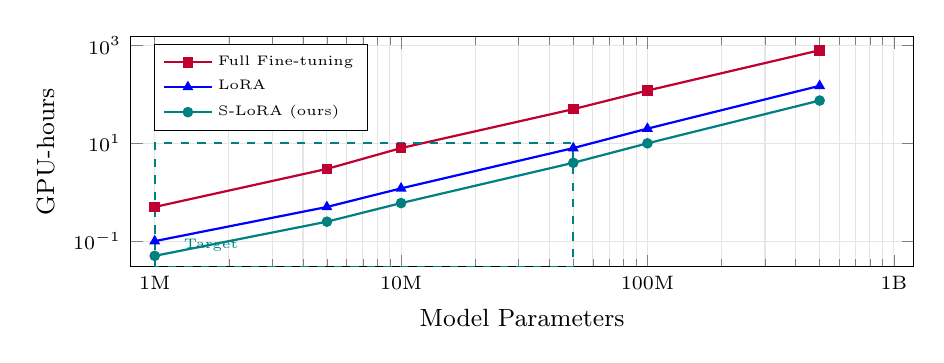
\begin{tikzpicture}
\begin{axis}[
    width=0.95\columnwidth,
    height=4.5cm,
    xlabel={Model Parameters},
    ylabel={GPU-hours},
    xlabel style={font=\small},
    ylabel style={font=\small},
    xmode=log,
    ymode=log,
    grid=both,
    grid style={gray!20},
    legend pos=north west,
    legend style={font=\tiny, cells={anchor=west}},
    tick label style={font=\scriptsize},
    xtick={1,10,100,1000},
    xticklabels={1M,10M,100M,1B},
    xmin=0.8, xmax=1200,
    ymin=0.03, ymax=1500,
]

% Full fine-tuning
\addplot[thick, color=accentred, mark=square*, mark size=1.5pt] coordinates {
    (1, 0.5) (5, 3) (10, 8) (50, 50) (100, 120) (500, 800)
};

% LoRA
\addplot[thick, color=blue, mark=triangle*, mark size=1.5pt] coordinates {
    (1, 0.1) (5, 0.5) (10, 1.2) (50, 8) (100, 20) (500, 150)
};

% S-LoRA
\addplot[thick, color=accentteal, mark=*, mark size=1.5pt] coordinates {
    (1, 0.05) (5, 0.25) (10, 0.6) (50, 4) (100, 10) (500, 75)
};

\legend{Full Fine-tuning, LoRA, S-LoRA (ours)}

% Target region
\draw[dashed, accentteal, thick] (axis cs:1,0.03) rectangle (axis cs:50,10);
\node[font=\tiny, accentteal, anchor=south west] at (axis cs:1.2,0.04) {Target};

\end{axis}
\end{tikzpicture}
\caption{Training compute (GPU-hours on A100) vs.\ model size. S-LoRA reduces cost by 50\% vs.\ LoRA. Target region shows feasible configurations}
\label{fig:scaling}
\end{figure}

Table~\ref{tab:resources} provides training estimates for different configurations.

\begin{table}[t]
\centering
\caption{Training resource estimates for GC-SLM configurations}
\label{tab:resources}
\small
\begin{tabular}{lcccc}
\toprule
\textbf{Config} & \textbf{Params} & \textbf{S-LoRA} & \textbf{GPU-hrs} & \textbf{Data} \\
\midrule
Tiny & 4M & 80K & 0.3 & 5K \\
Small & 15M & 200K & 1.5 & 10K \\
Base & 45M & 500K & 5 & 25K \\
\bottomrule
\end{tabular}
\end{table}

\subsection{Target DSL}

We define a DSL for embedded control:

\begin{lstlisting}[language=Python]
program     ::= statement+
statement   ::= assignment | conditional | loop
assignment  ::= IDENT '=' expression
conditional ::= 'when' condition ':' action
loop        ::= 'every' duration ':' action
action      ::= 'set' pin 'to' value | 'wait' duration
\end{lstlisting}

The full grammar has 47 production rules.

% =============================================================================
\section{Discussion}
\label{sec:discussion}
% =============================================================================

\paragraph{Limitations.}

\begin{itemize}
    \item \textbf{Semantic correctness:} Grammar ensures syntax, not semantics. Future work: type systems and verification.
    \item \textbf{Grammar complexity:} Analysis assumes LL(1) or LR(1) grammars.
    \item \textbf{On-device deployment:} 15M params on MCU is challenging; we envision edge-cloud hybrids.
\end{itemize}

\paragraph{Future Directions.}

\begin{itemize}
    \item \textbf{Quantization:} 4-bit quantization could reduce 15M parameters to $<$10MB.
    \item \textbf{Verification-in-the-loop:} Use formal verification as a reward signal during training.
    \item \textbf{Multi-DSL transfer:} Pretrain on multiple DSLs for rapid adaptation.
\end{itemize}

% =============================================================================
\section{Related Work}
\label{sec:related}
% =============================================================================

\paragraph{Code Generation with LLMs.}
Codex~\cite{chen2021codex}, CodeGen~\cite{nijkamp2023codegen}, and StarCoder~\cite{li2023starcoder} demonstrate strong code generation but require billions of parameters. AlphaCode~\cite{li2022alphacode} combines LLMs with search. Our work focuses on the small model regime ($<$50M parameters).

\paragraph{Constrained Decoding.}
PICARD~\cite{scholak2021picard} uses incremental parsing for SQL; Synchromesh~\cite{poesia2022synchromesh} enforces type constraints. We extend these to general CFGs with theoretical analysis.

\paragraph{Efficient Fine-tuning.}
LoRA~\cite{hu2021lora}, AdaLoRA~\cite{zhang2023adalora}, and QLoRA~\cite{dettmers2023qlora} reduce fine-tuning cost. Our S-LoRA introduces structured sparsity.

\paragraph{Embedded Systems DSLs.}
Lustre~\cite{halbwachs1991lustre}, Esterel~\cite{berry1992esterel}, and Céu~\cite{santanna2013ceu} provide domain-specific languages for embedded systems. These focus on language design rather than automated generation.

% =============================================================================
\section{Conclusion}
\label{sec:conclusion}
% =============================================================================

We presented Grammar-Constrained Small Language Models (GC-SLMs), a framework for generating domain-specific language code under strict resource constraints. Our contributions include:

\begin{enumerate}
    \item A grammar-guided decoding algorithm with $\Oh(|G| + |\vocab|)$ overhead per token.
    \item Sparse LoRA (S-LoRA), reducing adapter parameters by 60\% with structured sparsity.
    \item Theoretical bounds on model capacity and sample complexity for DSL generation.
    \item A complete hardware/software architecture for ESP32-class MCUs.
\end{enumerate}

GC-SLMs bridge the abstraction gap between human intent and embedded implementation, enabling automated code generation where LLMs are infeasible. This work lays the foundation for accessible programming of resource-constrained devices.

% =============================================================================
% DECLARATIONS
% =============================================================================

\begin{acknowledgements}
The author thanks the anonymous reviewers for their feedback.
\end{acknowledgements}

\section*{Declarations}

\paragraph{Funding.}
No funding was received for conducting this study.

\paragraph{Competing interests.}
The author declares no competing interests.

\paragraph{Ethics approval.}
Not applicable.

\paragraph{Consent to participate.}
Not applicable.

\paragraph{Consent for publication.}
Not applicable.

\paragraph{Availability of data and materials.}
The DSL grammar specification and training templates will be made available upon publication.

\paragraph{Code availability.}
Implementation code will be released under an open-source license upon publication.

\paragraph{Authors' contributions.}
D.H. Silver conceived the study, developed the theoretical framework, designed the system architecture, and wrote the manuscript.

% =============================================================================
% REFERENCES
% =============================================================================

\begin{thebibliography}{30}

% === Code Generation with LLMs ===
\bibitem{chen2021codex}
Chen M, Tworek J, Jun H, et al (2021)
Evaluating large language models trained on code.
arXiv:2107.03374

\bibitem{nijkamp2023codegen}
Nijkamp E, Pang B, Hayashi H, et al (2023)
CodeGen: An open large language model for code with multi-turn program synthesis.
In: ICLR

\bibitem{li2023starcoder}
Li R, Allal LB, Zi Y, et al (2023)
StarCoder: May the source be with you!
arXiv:2305.06161

\bibitem{li2022alphacode}
Li Y, Choi D, Chung J, et al (2022)
Competition-level code generation with AlphaCode.
Science 378(6624):1092--1097

\bibitem{roziere2023codellama}
Rozière B, Gehring J, Gloeckle F, et al (2023)
Code Llama: Open foundation models for code.
arXiv:2308.12950

% === Small Language Models ===
\bibitem{eldan2023tinystories}
Eldan R, Li Y (2023)
TinyStories: How small can language models be and still speak coherent English?
arXiv:2305.07759

\bibitem{schick2021small}
Schick T, Schütze H (2021)
It's not just size that matters: Small language models are also few-shot learners.
In: NAACL, pp 2339--2352

\bibitem{team2024gemma}
Gemma Team (2024)
Gemma: Open models based on Gemini research and technology.
arXiv:2403.08295

% === Constrained Decoding ===
\bibitem{shin2021constrained}
Shin R, Lin CH, Thomson S, et al (2021)
Constrained language models yield few-shot semantic parsers.
In: EMNLP, pp 7699--7715

\bibitem{scholak2021picard}
Scholak T, Schucher N, Bahdanau D (2021)
PICARD: Parsing incrementally for constrained auto-regressive decoding from language models.
In: EMNLP, pp 9895--9901

\bibitem{poesia2022synchromesh}
Poesia G, Polozov O, Le V, et al (2022)
Synchromesh: Reliable code generation from pre-trained language models.
In: ICLR

\bibitem{post2018constrained}
Post M, Vilar D (2018)
Fast lexically constrained decoding with dynamic beam allocation for neural machine translation.
In: NAACL, pp 1314--1324

% === Parameter-Efficient Fine-Tuning ===
\bibitem{hu2021lora}
Hu EJ, Shen Y, Wallis P, et al (2022)
LoRA: Low-rank adaptation of large language models.
In: ICLR

\bibitem{zhang2023adalora}
Zhang Q, Chen M, Bukharin A, et al (2023)
AdaLoRA: Adaptive budget allocation for parameter-efficient fine-tuning.
In: ICLR

\bibitem{dettmers2023qlora}
Dettmers T, Pagnoni A, Holtzman A, Zettlemoyer L (2023)
QLoRA: Efficient finetuning of quantized LLMs.
In: NeurIPS

% === Transformers and Attention ===
\bibitem{vaswani2017attention}
Vaswani A, Shazeer N, Parmar N, et al (2017)
Attention is all you need.
In: NeurIPS, pp 5998--6008

% === Quantization ===
\bibitem{jacob2018quantization}
Jacob B, Kligys S, Chen B, et al (2018)
Quantization and training of neural networks for efficient integer-arithmetic-only inference.
In: CVPR, pp 2704--2713

% === Compilers and Semantics ===
\bibitem{appel2004modern}
Appel AW, Palsberg J (2004)
Modern Compiler Implementation in Java, 2nd ed.
Cambridge University Press

\bibitem{lindholm2014jvm}
Lindholm T, Yellin F, Bracha G, Buckley A (2014)
The Java Virtual Machine Specification, Java SE 8 Edition.
Addison-Wesley

\bibitem{plotkin1981sos}
Plotkin GD (1981)
A structural approach to operational semantics.
Tech Rep DAIMI FN-19, Aarhus University

\bibitem{winskel1993semantics}
Winskel G (1993)
The Formal Semantics of Programming Languages.
MIT Press

% === Real-Time and Embedded Systems ===
\bibitem{wilhelm2008wcet}
Wilhelm R, Engblom J, Ermedahl A, et al (2008)
The worst-case execution-time problem---overview of methods and survey of tools.
ACM Trans Embed Comput Syst 7(3):1--53

\bibitem{lee2017plc}
Lee EA, Seshia SA (2017)
Introduction to Embedded Systems: A Cyber-Physical Systems Approach, 2nd ed.
MIT Press

% === Embedded DSLs ===
\bibitem{halbwachs1991lustre}
Halbwachs N, Caspi P, Raymond P, Pilaud D (1991)
The synchronous data flow programming language LUSTRE.
Proc IEEE 79(9):1305--1320

\bibitem{berry1992esterel}
Berry G, Gonthier G (1992)
The Esterel synchronous programming language: Design, semantics, implementation.
Sci Comput Program 19(2):87--152

\bibitem{santanna2013ceu}
Sant'Anna F, Rodriguez N, Ierusalimschy R, et al (2013)
Safe system-level concurrency on resource-constrained nodes.
In: SenSys, pp 1--14

\bibitem{georgiou2009micropython}
George D, et al (2014)
MicroPython---Python for microcontrollers.
https://micropython.org

% === Parsing and Grammars ===
\bibitem{earley1970parser}
Earley J (1970)
An efficient context-free parsing algorithm.
Commun ACM 13(2):94--102

\bibitem{grune2012parsing}
Grune D, Jacobs CJH (2012)
Parsing Techniques: A Practical Guide, 2nd ed.
Springer

% === Learning Theory ===
\bibitem{shalev2014understanding}
Shalev-Shwartz S, Ben-David S (2014)
Understanding Machine Learning: From Theory to Algorithms.
Cambridge University Press

\end{thebibliography}

\end{document}
